% ****************************************************************************************************
% Classification Procedural Model
% ****************************************************************************************************


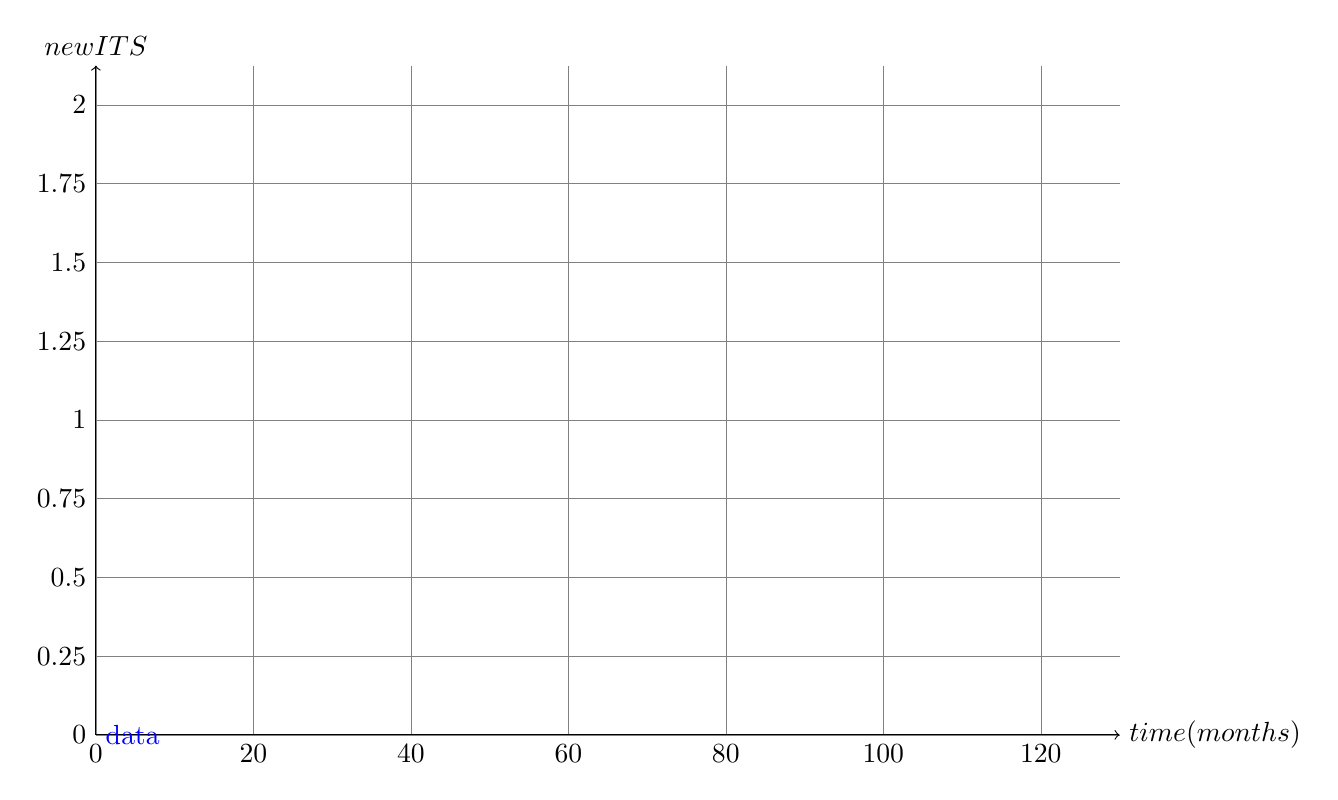
\begin{tikzpicture}[x=0.1cm,y=4cm]

  \def\xmin{0}
  \def\xmax{130}
  \def\ymin{0}
  \def\ymax{2.125}

  % grid
  \draw[style=help lines, ystep=0.25, xstep=20] (\xmin,\ymin) grid
  (\xmax,\ymax);

  % axes
  \draw[->] (\xmin,\ymin) -- (\xmax,\ymin) node[right] {$time (months)$};
  \draw[->] (\xmin,\ymin) -- (\xmin,\ymax) node[above] {$new ITS$};

  % xticks and yticks
  \foreach \x in {0,20,...,120}
    \node at (\x, \ymin) [below] {\x};
  \foreach \y in {0,0.25,...,2}
    \node at (\xmin,\y) [left] {\y};

  % plot the data from the file data.dat
  % smooth the curve and mark the data point with a dot
  \draw[color=blue] plot[smooth,mark=*,mark size=1pt] file {gfx/data.dat}
   node [right] {data};

  % generate and plot another a curve y = 0.1 x^2 + 2.5
  % this generates the files figure.parabola.gnuplot and figure.parabola.table 
  %\draw[color=red, domain=\xmin:\xmax] plot[id=parabola]
  %function{0.1*x**2 + 2.5} node [right] {$y=0.1\,x^2 + 2.5$};

\end{tikzpicture}
